% Options for packages loaded elsewhere
\PassOptionsToPackage{unicode}{hyperref}
\PassOptionsToPackage{hyphens}{url}
\documentclass[
]{article}
\usepackage{xcolor}
\usepackage{amsmath,amssymb}
\setcounter{secnumdepth}{5}
\usepackage{iftex}
\ifPDFTeX
  \usepackage[T1]{fontenc}
  \usepackage[utf8]{inputenc}
  \usepackage{textcomp} % provide euro and other symbols
\else % if luatex or xetex
  \usepackage{unicode-math} % this also loads fontspec
  \defaultfontfeatures{Scale=MatchLowercase}
  \defaultfontfeatures[\rmfamily]{Ligatures=TeX,Scale=1}
\fi
% \usepackage{lmodern}
\ifPDFTeX\else
  % xetex/luatex font selection
\fi
% Use upquote if available, for straight quotes in verbatim environments
\IfFileExists{upquote.sty}{\usepackage{upquote}}{}
\IfFileExists{microtype.sty}{% use microtype if available
  \usepackage[]{microtype}
  \UseMicrotypeSet[protrusion]{basicmath} % disable protrusion for tt fonts
}{}
\makeatletter
\@ifundefined{KOMAClassName}{% if non-KOMA class
  \IfFileExists{parskip.sty}{%
    \usepackage{parskip}
  }{% else
    \setlength{\parindent}{0pt}
    \setlength{\parskip}{6pt plus 2pt minus 1pt}}
}{% if KOMA class
  \KOMAoptions{parskip=half}}
\makeatother
\usepackage{color}
\usepackage{fancyvrb}
\newcommand{\VerbBar}{|}
\newcommand{\VERB}{\Verb[commandchars=\\\{\}]}
\DefineVerbatimEnvironment{Highlighting}{Verbatim}{commandchars=\\\{\}}
% Add ',fontsize=\small' for more characters per line
\newenvironment{Shaded}{}{}
\newcommand{\AlertTok}[1]{\textcolor[rgb]{1.00,0.00,0.00}{\textbf{#1}}}
\newcommand{\AnnotationTok}[1]{\textcolor[rgb]{0.38,0.63,0.69}{\textbf{\textit{#1}}}}
\newcommand{\AttributeTok}[1]{\textcolor[rgb]{0.49,0.56,0.16}{#1}}
\newcommand{\BaseNTok}[1]{\textcolor[rgb]{0.25,0.63,0.44}{#1}}
\newcommand{\BuiltInTok}[1]{\textcolor[rgb]{0.00,0.50,0.00}{#1}}
\newcommand{\CharTok}[1]{\textcolor[rgb]{0.25,0.44,0.63}{#1}}
\newcommand{\CommentTok}[1]{\textcolor[rgb]{0.38,0.63,0.69}{\textit{#1}}}
\newcommand{\CommentVarTok}[1]{\textcolor[rgb]{0.38,0.63,0.69}{\textbf{\textit{#1}}}}
\newcommand{\ConstantTok}[1]{\textcolor[rgb]{0.53,0.00,0.00}{#1}}
\newcommand{\ControlFlowTok}[1]{\textcolor[rgb]{0.00,0.44,0.13}{\textbf{#1}}}
\newcommand{\DataTypeTok}[1]{\textcolor[rgb]{0.56,0.13,0.00}{#1}}
\newcommand{\DecValTok}[1]{\textcolor[rgb]{0.25,0.63,0.44}{#1}}
\newcommand{\DocumentationTok}[1]{\textcolor[rgb]{0.73,0.13,0.13}{\textit{#1}}}
\newcommand{\ErrorTok}[1]{\textcolor[rgb]{1.00,0.00,0.00}{\textbf{#1}}}
\newcommand{\ExtensionTok}[1]{#1}
\newcommand{\FloatTok}[1]{\textcolor[rgb]{0.25,0.63,0.44}{#1}}
\newcommand{\FunctionTok}[1]{\textcolor[rgb]{0.02,0.16,0.49}{#1}}
\newcommand{\ImportTok}[1]{\textcolor[rgb]{0.00,0.50,0.00}{\textbf{#1}}}
\newcommand{\InformationTok}[1]{\textcolor[rgb]{0.38,0.63,0.69}{\textbf{\textit{#1}}}}
\newcommand{\KeywordTok}[1]{\textcolor[rgb]{0.00,0.44,0.13}{\textbf{#1}}}
\newcommand{\NormalTok}[1]{#1}
\newcommand{\OperatorTok}[1]{\textcolor[rgb]{0.40,0.40,0.40}{#1}}
\newcommand{\OtherTok}[1]{\textcolor[rgb]{0.00,0.44,0.13}{#1}}
\newcommand{\PreprocessorTok}[1]{\textcolor[rgb]{0.74,0.48,0.00}{#1}}
\newcommand{\RegionMarkerTok}[1]{#1}
\newcommand{\SpecialCharTok}[1]{\textcolor[rgb]{0.25,0.44,0.63}{#1}}
\newcommand{\SpecialStringTok}[1]{\textcolor[rgb]{0.73,0.40,0.53}{#1}}
\newcommand{\StringTok}[1]{\textcolor[rgb]{0.25,0.44,0.63}{#1}}
\newcommand{\VariableTok}[1]{\textcolor[rgb]{0.10,0.09,0.49}{#1}}
\newcommand{\VerbatimStringTok}[1]{\textcolor[rgb]{0.25,0.44,0.63}{#1}}
\newcommand{\WarningTok}[1]{\textcolor[rgb]{0.38,0.63,0.69}{\textbf{\textit{#1}}}}
\usepackage{longtable,booktabs,array}
\newcounter{none} % for unnumbered tables
\usepackage{calc} % for calculating minipage widths
% Correct order of tables after \paragraph or \subparagraph
\usepackage{etoolbox}
\makeatletter
\patchcmd\longtable{\par}{\if@noskipsec\mbox{}\fi\par}{}{}
\makeatother
% Allow footnotes in longtable head/foot
\IfFileExists{footnotehyper.sty}{\usepackage{footnotehyper}}{\usepackage{footnote}}
\makesavenoteenv{longtable}
\usepackage{graphicx}
\makeatletter
\newsavebox\pandoc@box
\newcommand*\pandocbounded[1]{% scales image to fit in text height/width
  \sbox\pandoc@box{#1}%
  \Gscale@div\@tempa{\textheight}{\dimexpr\ht\pandoc@box+\dp\pandoc@box\relax}%
  \Gscale@div\@tempb{\linewidth}{\wd\pandoc@box}%
  \ifdim\@tempb\p@<\@tempa\p@\let\@tempa\@tempb\fi% select the smaller of both
  \ifdim\@tempa\p@<\p@\scalebox{\@tempa}{\usebox\pandoc@box}%
  \else\usebox{\pandoc@box}%
  \fi%
}
% Set default figure placement to htbp
\def\fps@figure{htbp}
\makeatother
\setlength{\emergencystretch}{3em} % prevent overfull lines
\providecommand{\tightlist}{%
  \setlength{\itemsep}{0pt}\setlength{\parskip}{0pt}}
\usepackage[]{natbib}
\bibliographystyle{plainnat}
\makeatletter
\@ifpackageloaded{subcaption}{}{\usepackage{subcaption}}
\@ifpackageloaded{caption}{}{\usepackage{caption}}
\captionsetup[subfigure]{margin=0.5em}
\AtBeginDocument{%
\renewcommand*\figurename{Figure}
\renewcommand*\tablename{Table}
}
\AtBeginDocument{%
\renewcommand*\listfigurename{List of Figures}
\renewcommand*\listtablename{List of Tables}
}
\newcounter{pandoccrossref@subfigures@footnote@counter}
\newenvironment{pandoccrossrefsubfigures}{%
\setcounter{pandoccrossref@subfigures@footnote@counter}{0}
\begin{figure}\centering%
\gdef\global@pandoccrossref@subfigures@footnotes{}%
\DeclareRobustCommand{\footnote}[1]{\footnotemark%
\stepcounter{pandoccrossref@subfigures@footnote@counter}%
\ifx\global@pandoccrossref@subfigures@footnotes\empty%
\gdef\global@pandoccrossref@subfigures@footnotes{{##1}}%
\else%
\g@addto@macro\global@pandoccrossref@subfigures@footnotes{, {##1}}%
\fi}}%
{\end{figure}%
\addtocounter{footnote}{-\value{pandoccrossref@subfigures@footnote@counter}}
\@for\f:=\global@pandoccrossref@subfigures@footnotes\do{\stepcounter{footnote}\footnotetext{\f}}%
\gdef\global@pandoccrossref@subfigures@footnotes{}}
\@ifpackageloaded{float}{}{\usepackage{float}}
\floatstyle{ruled}
\@ifundefined{c@chapter}{\newfloat{codelisting}{h}{lop}}{\newfloat{codelisting}{h}{lop}[chapter]}
\floatname{codelisting}{Listing}
\newcommand*\listoflistings{\listof{codelisting}{List of Listings}}
\makeatother
\usepackage{bookmark}
\IfFileExists{xurl.sty}{\usepackage{xurl}}{} % add URL line breaks if available
\urlstyle{same}
% fallback for those not using the hyperref driver hyperxmp:
\makeatletter
\@ifundefined{xmpquote}{\newcommand{\xmpquote}[1]{#1}}{}
\makeatother
\hypersetup{
  colorlinks=true,linkcolor=red,urlcolor=red,citecolor=red,anchorcolor=red,filecolor=red,
  pdfcreator={LaTeX via pandoc}}

\author{}
\date{}

\IfFileExists{seqsplit.sty}{\usepackage{seqsplit}}{\newcommand{\seqsplit}[1]{#1}}
\protected\def\breakseq#1{\seqsplit{#1}}
\protected\def\breaktt#1{\begingroup\ttfamily\seqsplit{#1}\endgroup}
\title{Exploratory Data Analysis: A Reproducible Notebook Template}
\author{Daniel Ari Friedman\\\footnotesize{Active Inference Institute}\\\footnotesize{\texttt{daniel@activeinference.institute}}\\\footnotesize{\href{https://orcid.org/0000-0001-6232-9096}{ORCID: 0000-0001-6232-9096}}}
\date{\today}

% Core mathematics
\usepackage{amsmath}
\usepackage{amssymb}
\usepackage{amsfonts}
\usepackage{amsthm}

% Document layout
\usepackage{geometry}
\geometry{margin=0.25in}
\usepackage{float}
\usepackage{graphicx}

% Tables
\usepackage{booktabs}
\usepackage{longtable}
\usepackage{array}

% Algorithm typesetting (available for pseudocode if a fork needs it)
\usepackage[ruled,vlined,linesnumbered]{algorithm2e}

% Code listings
\usepackage{listings}

% Typography and formatting
\usepackage{microtype}
\usepackage{xcolor}
\usepackage[binary-units]{siunitx}

% Cross-references and citations
\usepackage{hyperref}
\hypersetup{
    colorlinks=true,
    allcolors=red
}
\usepackage[capitalise,noabbrev]{cleveref}
\usepackage{natbib}

% ── Unicode-capable mono font for code listings ──────────────────────
% JuliaMono (TeX Live 2026) covers the full math/Greek glyph set used in
% scientific code blocks; the default lmmono lacks \alpha/\mu/\partial/\nabla.
%
% The hardcoded TeX Live 2026 path below is portable to most macOS / Linux
% TeX Live installs that placed JuliaMono under the default texmf-dist path.
% If your TeX Live version differs (e.g., 2025, 2027) or your distribution
% installs fonts elsewhere, comment out the explicit Path = line — fontspec
% will then search the system font path. If JuliaMono is not installed at
% all, comment out the whole block; xelatex falls back to lmmono with
% reduced Unicode coverage but the document still compiles.
\usepackage{fontspec}
\setmonofont{JuliaMono-Regular}[
  Path           = /usr/local/texlive/2026/texmf-dist/fonts/truetype/public/juliamono/,
  Extension      = .ttf,
  UprightFont    = *,
  BoldFont       = JuliaMono-Bold,
  ItalicFont     = JuliaMono-RegularItalic,
  BoldItalicFont = JuliaMono-BoldItalic,
  Scale          = MatchLowercase,
]

% Math font for unicode-math: Latin Modern Math (TeX Live) has full BMP
% coverage including U+2223 (\mid), U+226A/226B (\ll/\gg), and the Greek/
% blackboard letters used in equations. Without an explicit \setmathfont,
% unicode-math falls back to lmroman text font which lacks several glyphs
% and emits "Missing character" warnings on every \mid in math mode.
\setmathfont{latinmodern-math.otf}

\begin{document}

\begin{titlepage}
\centering
\vspace*{2cm}
{\LARGE\bfseries Exploratory Data Analysis: A Reproducible Notebook Template\par}
\vspace{0.75em}
{\large Notebook-to-Tested-Source Extraction for Computational Research\par}
\vfill
\makeatletter
{\@author\par}
\vspace{1em}
{\@date\par}
\makeatother
\vfill
\end{titlepage}
\thispagestyle{empty}
\tableofcontents
\newpage


\section{Abstract}\label{sec:abstract}

Exploratory data analysis (EDA) is the most common entry point in
applied research, yet it is also where reproducibility most often breaks
down: logic accumulates in notebook cells that are never tested and
quietly drift from the prose describing them. This paper presents the
\textbf{computational-notebook exemplar} of the
\href{https://github.com/docxology/template}{Research Project Template}:
an interactive walkthrough notebook
(\breaktt{projects/templates/template\_eda\_notebook/notebooks/eda\_walkthrough.ipynb})
that imports a small, fully-tested EDA library rather than carrying
logic in its cells.

We ship a deterministic dataset (\breaktt{data/measurements.csv}) with a
designed correlation structure and a handful of missing values, then
load, clean, summarize, correlate, and visualize it entirely through
tested functions in \texttt{src/eda/}. The library is side-effect-free
--- no plotting and no file I/O --- and standalone (numpy and pandas
only), so it is covered above the 90\% project gate and reused
identically from the notebook, the thin analysis script
(\breaktt{scripts/eda\_analysis.py}), and this manuscript.

Contributions are \textbf{methodological} and \textbf{architectural}. On
the methods side, we walk the canonical first EDA pass: surface
missingness explicitly rather than imputing it, compute per-column
descriptive statistics and per-group means, and rank features by Pearson
correlation. On the architecture side, we demonstrate the
notebook-to-tested-source extraction workflow --- explore fast in a
cell, and the moment a computation matters, move it into the library
behind a failing test --- verified by a zero-mock suite and a structural
notebook-binding check (sec.~\ref{sec:reproducibility}).

\newpage

\section{Introduction}\label{sec:introduction}

This \breaktt{template\_eda\_notebook} serves as the
exploratory-data-analysis exemplar for the
\href{https://github.com/docxology/template}{Research Project Template}
ecosystem, demonstrating how a computational notebook can stay
reproducible by delegating every computation to a fully-tested library.
The prose, the labelled figures, and the summary table are all produced
through an auditable custody chain: a deterministic dataset, tested
functions in \texttt{src/eda/}, a thin analysis script, and multi-format
rendering.

\subsection{Why exploratory data
analysis}\label{why-exploratory-data-analysis}

EDA --- the work of getting to know a dataset before committing to a
model --- is where most research projects actually begin: load the data,
see how much is missing, look at distributions, and check which
variables move together. It is fast and interactive by nature, which is
exactly why it tends to live in notebooks. The hazard is that the
interactive convenience of a notebook cell is also a trap: a one-off
\breaktt{df.groupby(...).mean()} becomes load-bearing, never gets a test,
and silently disagrees with the figure two cells down after the data
changes.

\subsection{The notebook -\textgreater{} tested src extraction
workflow}\label{the-notebook---tested-src-extraction-workflow}

This exemplar teaches one discipline: \textbf{explore in a cell, then
extract to a tested library the moment a computation matters.}
Concretely:

\begin{enumerate}
\def\labelenumi{\arabic{enumi}.}
\tightlist
\item
  The walkthrough notebook (\breaktt{notebooks/eda\_walkthrough.ipynb})
  imports from \texttt{src} and calls tested functions; it contains no
  business logic of its own.
\item
  Each analytical step --- loading, cleaning, summarizing, correlating,
  preparing figure data --- is a typed, documented function in
  \texttt{src/eda/} with a test that asserts an exact numeric property.
\item
  A thin script (\breaktt{scripts/eda\_analysis.py}) runs the same
  pipeline headless and writes the figures and a summary CSV to
  \texttt{output/}.
\end{enumerate}

\subsection{Template architecture
context}\label{template-architecture-context}

The project sits on the repository's three pillars:

\begin{enumerate}
\def\labelenumi{\arabic{enumi}.}
\tightlist
\item
  \textbf{\texttt{src/eda/} library}: pure pandas/numpy data transforms
  --- no plotting, no file I/O, no \texttt{infrastructure} imports. This
  purity is what makes the library forkable and trivially testable.
\item
  \textbf{\texttt{tests/} framework}: a zero-mock suite that exercises
  the library against the shipped CSV and tiny real frames, plus a
  structural check that the notebook's imports bind to the library's
  public surface.
\item
  \textbf{\texttt{docs/} knowledge base}: architectural guidelines, the
  testing philosophy, and the operational rules that govern agents
  editing this tree.
\end{enumerate}

\subsection{The dataset}\label{the-dataset}

We analyze a small synthetic cohort of subject measurements --- height
(cm), weight (kg), and resting heart rate (bpm) across three groups ---
generated with a fixed seed so every statistic in sec.~\ref{sec:results}
is reproducible. The data is shaped so that weight depends positively on
height (a strong, easy-to-see correlation) while resting heart rate is
only weakly related, and a few cells are left blank to exercise the
missing-data path honestly.

\subsection{Reader's guide to the
manuscript}\label{readers-guide-to-the-manuscript}

\begin{itemize}
\tightlist
\item
  \textbf{sec.~\ref{sec:methodology}} ties each EDA step to its function
  in \texttt{src/eda/}.
\item
  \textbf{sec.~\ref{sec:results}} is figure-centric: each panel names
  the figure-data preparer that produced it.
\item
  \textbf{sec.~\ref{sec:experimental_setup}} lists the dataset schema
  and software environment.
\item
  \textbf{sec.~\ref{sec:reproducibility}} records the artifact inventory
  and the exact commands to regenerate everything.
\item
  \textbf{sec.~\ref{sec:scope}} states scope and related literature so
  the exemplar is not mistaken for a general-purpose EDA toolkit.
\end{itemize}

\newpage

\section{Methodology}\label{sec:methodology}

This section maps each step of the exploratory analysis to the tested
function that implements it. Every function lives in \texttt{src/eda/},
takes a \breaktt{pandas.DataFrame} in, and returns data out --- no
plotting, no file I/O --- so the notebook, the analysis script, and this
manuscript all reach the same code.

\subsection{Dataset loading and
schema}\label{dataset-loading-and-schema}

\breaktt{src/eda/dataset.py::load\_dataset()} reads the shipped CSV and
coerces the numeric columns with
\breaktt{pandas.to\_numeric(errors="coerce")}. Coercion is deliberate: a
blank or non-numeric cell becomes \texttt{NaN} rather than raising or
being silently dropped, so missingness is \emph{surfaced} and handled in
an explicit later step. The column roles are declared once in a frozen
\texttt{DatasetSchema} (an identifier column, a categorical group
column, and three numeric features), which downstream functions consult
instead of re-sniffing dtypes.

\subsection{Cleaning: explicit, reported row
removal}\label{cleaning-explicit-reported-row-removal}

\breaktt{src/eda/cleaning.py::clean\_dataset()} drops any row missing a
numeric feature and returns a \texttt{CleaningReport} recording how many
rows entered, how many remained, and how many were dropped. This
exemplar makes a deliberate choice --- listwise deletion with a visible
count --- rather than imputation, because a first EDA pass should
\emph{see} the missingness, not paper over it. A separate
\breaktt{normalize\_numeric()} z-score standardizes the numeric columns
(mean 0, sample standard deviation 1), with a guard that maps a constant
or single-row column to zeros instead of producing
\texttt{inf}/\texttt{NaN}.

\subsection{Descriptive statistics}\label{descriptive-statistics}

\breaktt{src/eda/statistics.py::summary\_statistics()} returns one
\texttt{ColumnSummary} per numeric column --- count of non-missing
observations, mean, sample standard deviation, minimum, median, and
maximum --- computed with real pandas aggregation.
\texttt{group\_means()} returns the mean of each numeric feature grouped
by the categorical column, sorted by group name for deterministic
output.

\subsection{Correlation structure}\label{correlation-structure}

\breaktt{src/eda/correlation.py::correlation\_matrix()} returns the
Pearson correlation matrix of the numeric columns \citep{tukey1977eda}.
The companion \breaktt{strongest\_pairs(matrix,\ top\_n)} ranks the
distinct off-diagonal feature pairs by absolute correlation while
preserving sign --- usually the single most useful artifact of a first
pass, because it points directly at the relationships worth
investigating. Each unordered pair appears exactly once.

\subsection{Figure-data preparers}\label{figure-data-preparers}

Plotting is kept out of the library entirely.
\breaktt{src/eda/figures.py} returns \emph{plot-ready data structures}
--- bin counts and edges for a histogram, a square value grid plus
labels for a correlation heatmap, and sorted category counts for a bar
chart --- as frozen dataclasses of plain numbers. The thin analysis
script (\breaktt{scripts/eda\_analysis.py}) and notebook cells consume
these structures and call matplotlib. This keeps the library importable
on a headless machine and makes every preparer testable without a
display backend.

\subsection{Zero-mock testing
methodology}\label{zero-mock-testing-methodology}

The project is governed by a strict zero-mock policy, evaluated by
running
\breaktt{uv\ run\ pytest\ projects/templates/template\_eda\_notebook/tests}
during the build.

\begin{enumerate}
\def\labelenumi{\arabic{enumi}.}
\tightlist
\item
  \textbf{Library tests} exercise every public function against the
  shipped CSV or a tiny hand-built frame with values chosen so the
  expected statistic is exact (e.g.~\breaktt{weight\ =\ 2\ *\ height}
  gives a correlation of exactly \texttt{+1.0}). No
  \texttt{unittest.mock}, no \texttt{MagicMock}, no \texttt{@patch}.
\item
  \textbf{Script test} runs \texttt{run\_eda()} against a temporary
  output root and asserts that real PNG figures and a real summary CSV
  are written.
\item
  \textbf{Notebook test} parses the real \texttt{.ipynb} and asserts it
  is valid nbformat, that every name imported \texttt{from\ src} exists
  in the library's public surface, and that no cell defines its own
  \texttt{def}/\texttt{class}.
\item
  \textbf{Coverage gate}: CI enforces a \texorpdfstring{\textgreater{}=}{>=}90\% statement-coverage gate on
  \breaktt{projects/templates/template\_eda\_notebook/src/}; the live
  figure is tracked in
  \href{../../../../docs/_generated/COUNTS.md}{\breaktt{docs/\_generated/COUNTS.md}}.
\end{enumerate}

\subsection{Figure generation
contract}\label{figure-generation-contract}

Each figure in \texttt{03\_results.md} maps to a figure-data preparer in
\breaktt{src/eda/figures.py}: \texttt{histogram\_data} \texorpdfstring{\ensuremath{\to}}{->} height
histogram, \breaktt{correlation\_heatmap\_data} \texorpdfstring{\ensuremath{\to}}{->} feature-correlation
heatmap, and \breaktt{group\_count\_data} \texorpdfstring{\ensuremath{\to}}{->} per-group row counts.
Captions name the preparer and the key parameters (bin count, value
range) so reviewers can navigate from the PDF to the code without
inferring hidden defaults.

\newpage

\section{Results}\label{sec:results}

This section presents the exploratory analysis of the shipped dataset.
Every figure and the summary table are produced by the thin analysis
script
(\href{https://github.com/docxology/template/blob/main/projects/templates/template_eda_notebook/scripts/eda_analysis.py}{\breaktt{scripts/eda\_analysis.py}}),
which calls the tested figure-data preparers in
\breaktt{src/eda/figures.py}. Running the script regenerates the figures
under \texttt{../figures/} and the summary CSV under
\texttt{output/data/}; the prose below describes what those artifacts
show.

\subsection{Dataset and missingness}\label{dataset-and-missingness}

The dataset contains 120 subject records across three groups
(\texttt{alpha}, \texttt{beta}, \texttt{gamma}) with three numeric
features: height (cm), weight (kg), and resting heart rate (bpm). A
small number of cells are blank by design. \texttt{load\_dataset()}
preserves these as \texttt{NaN}; \texttt{clean\_dataset()} then drops
rows missing any numeric feature and reports the count. With the shipped
data, four rows are removed, leaving a complete-case dataset for the
analysis below.

\subsection{Distributions}\label{distributions}

fig.~\ref{fig:height_histogram} shows the distribution of height across
the complete-case dataset, binned by \breaktt{histogram\_data()} and
plotted by the analysis script.

\begin{figure}
\centering
\pandocbounded{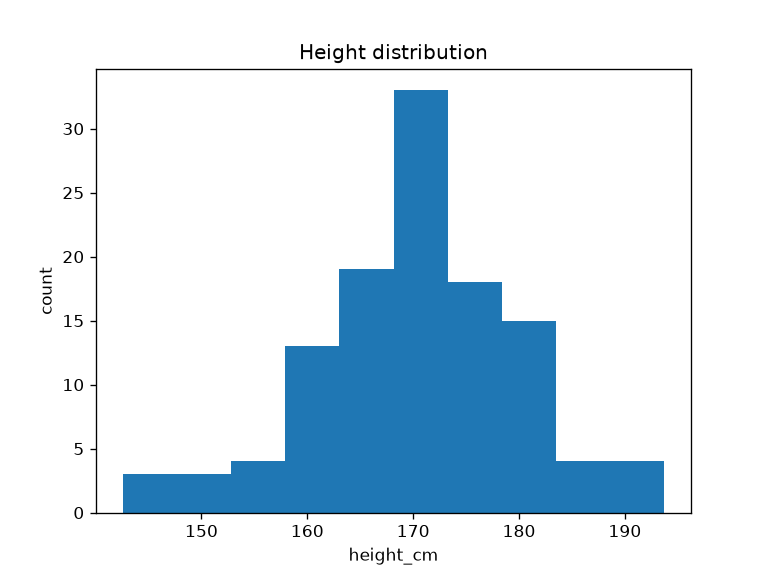
\includegraphics[keepaspectratio,alt={Height distribution: bin counts produced by histogram\_data(frame, "height\_cm", bins=10) in src/eda/figures.py and plotted as a bar chart by scripts/eda\_analysis.py. The bin counts sum to the number of complete-case rows; the shape is the roughly bell-shaped spread expected from the generating process.}]{../figures/height_histogram.png}}
\caption{Height distribution: bin counts produced by
\protect\breaktt{histogram\_data(frame,\ "height\_cm",\ bins=10)} in
\protect\breaktt{src/eda/figures.py} and plotted as a bar chart by
\protect\breaktt{scripts/eda\_analysis.py}. The bin counts sum to the
number of complete-case rows; the shape is the roughly bell-shaped
spread expected from the generating
process.}\label{fig:height_histogram}
\end{figure}

\subsection{Group composition}\label{group-composition}

fig.~\ref{fig:group_counts} reports how many complete-case rows fall in
each group, computed by \breaktt{group\_count\_data()} (labels sorted for
deterministic output).

\begin{figure}
\centering
\pandocbounded{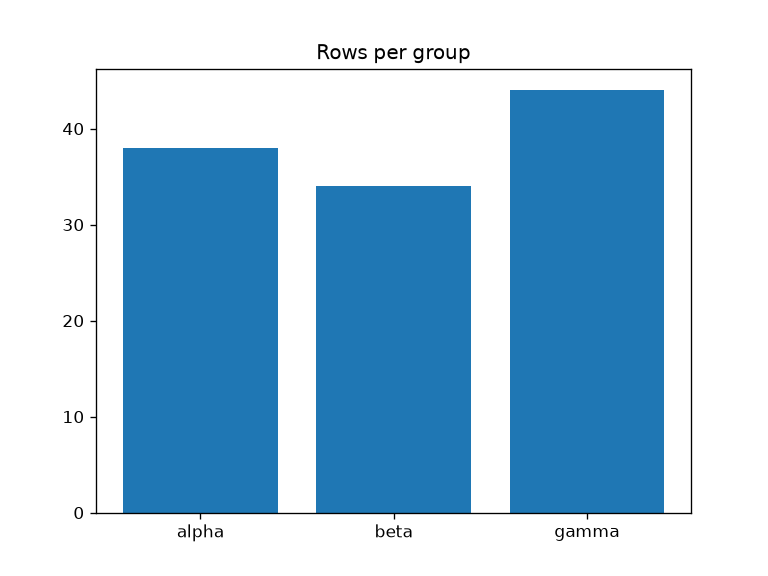
\includegraphics[keepaspectratio,alt={Rows per group: sorted category labels and aligned counts from group\_count\_data(). The three groups are of comparable, though not identical, size; the counts sum to the complete-case row total.}]{../figures/group_counts.png}}
\caption{Rows per group: sorted category labels and aligned counts from
\protect\breaktt{group\_count\_data()}. The three groups are of
comparable, though not identical, size; the counts sum to the
complete-case row total.}\label{fig:group_counts}
\end{figure}

\subsection{Correlation structure}\label{correlation-structure-1}

fig.~\ref{fig:correlation_heatmap} visualizes the Pearson correlation
matrix of the three numeric features, computed by
\breaktt{correlation\_matrix()} and prepared for the heatmap by
\breaktt{correlation\_heatmap\_data()}. The diagonal is unity by
construction and the matrix is symmetric.

\begin{figure}
\centering
\pandocbounded{\includegraphics[keepaspectratio,alt={Feature correlation heatmap: values from correlation\_heatmap\_data() (which wraps correlation\_matrix(method="pearson")) rendered with a diverging colour map on the fixed range {[}-1, 1{]}. Height and weight are strongly positively correlated; resting heart rate is only weakly related to the other two.}]{../figures/correlation_heatmap.png}}
\caption{Feature correlation heatmap: values from
\protect\breaktt{correlation\_heatmap\_data()} (which wraps
\protect\breaktt{correlation\_matrix(method="pearson")}) rendered with a
diverging colour map on the fixed range \([-1, 1]\). Height and weight
are strongly positively correlated; resting heart rate is only weakly
related to the other two.}\label{fig:correlation_heatmap}
\end{figure}

\breaktt{strongest\_pairs(matrix,\ top\_n=3)} ranks the distinct feature
pairs by absolute correlation while preserving sign. On the shipped data
the dominant relationship is \textbf{height about  weight} (a
strong positive correlation, by design), followed by the comparatively
weak \textbf{height about  resting heart rate} (slightly
negative) and \textbf{weight about  resting heart rate}. This
ranking is the single most useful artifact of the first pass: it points
directly at the relationship worth modelling next.

\subsection{Summary statistics}\label{summary-statistics}

The analysis script writes a per-column summary table to
\breaktt{output/data/summary\_statistics.csv} from
\breaktt{summary\_statistics()}. Each row reports the count of
non-missing observations, mean, sample standard deviation, minimum,
median, and maximum for one numeric feature.

\begin{longtable}[]{@{}ll@{}}
\caption{Summary-statistics table written by the analysis script from
\protect\breaktt{src/eda/statistics.py::summary\_statistics()}. The
concrete numbers are reproduced verbatim by running the script --- the
manuscript intentionally does not transcribe volatile values, so prose
and CSV cannot drift.}\label{tbl:summary_statistics}\tabularnewline
\toprule\noalign{}
Column & Reported statistics \\
\midrule\noalign{}
\endfirsthead
\toprule\noalign{}
Column & Reported statistics \\
\midrule\noalign{}
\endhead
\bottomrule\noalign{}
\endlastfoot
\texttt{height\_cm} & count, mean, std, min, median, max \\
\texttt{weight\_kg} & count, mean, std, min, median, max \\
\texttt{resting\_hr\_bpm} & count, mean, std, min, median, max \\
\end{longtable}

\texttt{group\_means()} complements this with the mean of each numeric
feature within each group; the three group means for height are close
but not equal, reflecting the mild group structure in the generating
process.

\subsection{Validation}\label{validation}

The analysis was validated through the zero-mock \texttt{tests/} suite:

\begin{itemize}
\tightlist
\item
  \textbf{Library tests} assert exact statistics, correlation signs, and
  bin counts against the shipped CSV and hand-built frames.
\item
  \textbf{Script test} runs \texttt{run\_eda()} against a temporary
  output root and confirms real PNG figures and a real summary CSV are
  written.
\item
  \textbf{Notebook test} confirms the walkthrough notebook binds to the
  library's public surface and carries no logic in its cells.
\end{itemize}

All tests pass with coverage exceeding the 90\% project gate, with no
mocks.

\subsection{Discussion}\label{discussion}

The results confirm the EDA workflow end to end: missingness is surfaced
and removed with an explicit count, distributions and group composition
are read straight from tested preparers, and the correlation ranking
recovers the designed height--weight relationship. The same functions
back the interactive notebook, the headless script, and this manuscript
--- which is the architectural point of the exemplar. Because every
number is produced by a tested function and regenerated on demand, the
prose here describes structure and provenance rather than transcribing
values that would drift the moment the data changed.

\newpage

\section{Conclusion}\label{sec:conclusion}

This study demonstrated a complete, reproducible
exploratory-data-analysis pipeline driven from a computational notebook
backed by a tested library. It validates a simple proposition: a
notebook stays trustworthy when its cells call tested code instead of
carrying logic.

\subsection{Exemplar achievements}\label{exemplar-achievements}

Operating as the EDA exemplar for the Research Project Template
methodology, the project deployed the three foundational pillars:

\begin{enumerate}
\def\labelenumi{\arabic{enumi}.}
\tightlist
\item
  \textbf{\texttt{src/eda/} library}: pure pandas/numpy data transforms
  --- loading, cleaning, summary statistics, correlation, and
  figure-data preparation --- with no plotting, no file I/O, and no
  \texttt{infrastructure} imports.
\item
  \textbf{\texttt{tests/} integrity}: a zero-mock suite over the shipped
  dataset and hand-built frames, plus a structural notebook-binding
  check, all under a \texorpdfstring{\textgreater{}=}{>=}90\% project coverage gate.
\item
  \textbf{\texttt{docs/} knowledge operations}: architecture, testing
  philosophy, and operational rules that keep the notebook, script, and
  manuscript aligned.
\end{enumerate}

\subsection{Technical contributions}\label{technical-contributions}

\subsubsection{The notebook -\textgreater{} tested src extraction
workflow}\label{the-notebook---tested-src-extraction-workflow-1}

The hallmark of this exemplar is the discipline it teaches: explore fast
in a cell, and the moment a computation matters, move it into
\texttt{src/eda/} behind a failing test. The walkthrough notebook
imports only the library's public surface and defines no functions of
its own, a property the test suite enforces structurally so it cannot
regress.

\subsubsection{Honest handling of imperfect
data}\label{honest-handling-of-imperfect-data}

The loader surfaces missing values as \texttt{NaN} instead of silently
imputing them, and \texttt{clean\_dataset()} removes incomplete rows
with an explicit count. This makes data quality a visible, testable
property of the first pass rather than a hidden assumption.

\subsection{Key insights}\label{key-insights}

\begin{enumerate}
\def\labelenumi{\arabic{enumi}.}
\tightlist
\item
  \textbf{Reproducibility follows from testing fidelity}: every number
  in sec.~\ref{sec:results} is produced by a tested function and
  regenerated on demand, so prose and artifacts cannot drift.
\item
  \textbf{Purity enables reuse}: because \texttt{src/eda/} returns
  plot-ready data and never touches a display backend, the same
  functions serve the notebook, the headless script, and the manuscript.
\item
  \textbf{Missingness is information}: reporting dropped rows beats
  imputing them away in an exploratory pass.
\end{enumerate}

\subsection{Future extensions}\label{future-extensions}

This foundation could be extended to:

\begin{itemize}
\tightlist
\item
  \textbf{Richer cleaning}: typed imputation strategies behind tested
  functions, with the report recording which strategy ran.
\item
  \textbf{More figure preparers}: box plots, pair plots, and per-group
  overlays --- each a tested data preparer plus a thin plotting call.
\item
  \textbf{Larger / external datasets}: swap the shipped CSV for a real
  dataset by pointing \breaktt{load\_dataset(path=...)} at it while
  keeping the schema contract.
\end{itemize}

\subsection{Final assessment}\label{final-assessment}

The \breaktt{template\_eda\_notebook} tree is the canonical reference for
how an exploratory notebook, a thin analysis script, a tested library,
and a manuscript stay synchronized across rebuilds. The pipeline
produced the figures referenced in sec.~\ref{sec:results}, wrote
\breaktt{output/data/summary\_statistics.csv}, and rendered this markdown
together with \texttt{config.yaml} into PDF.

\newpage

\section{Experimental Setup}\label{sec:experimental_setup}

This section details the dataset, schema, and software environment used
to produce the results. The exemplar deliberately avoids manuscript
token injection: concrete numbers are reproduced by running the analysis
script, and the figures are regenerated from tested code, so nothing
here can silently drift from a hardcoded value.

\subsection{Dataset}\label{dataset}

The analysis uses a shipped, deterministic CSV fixture
(\breaktt{data/measurements.csv}) generated once with a fixed NumPy seed.
It contains 120 subject records with the following columns:

{\def\LTcaptype{none} % do not increment counter
\begin{longtable}[]{@{}lll@{}}
\toprule\noalign{}
Column & Role & Type \\
\midrule\noalign{}
\endhead
\bottomrule\noalign{}
\endlastfoot
\texttt{subject\_id} & per-row identifier & string \\
\texttt{group} & categorical group (\texttt{alpha}, \texttt{beta},
\texttt{gamma}) & string \\
\texttt{height\_cm} & numeric feature & float \\
\texttt{weight\_kg} & numeric feature & float \\
\texttt{resting\_hr\_bpm} & numeric feature & float \\
\end{longtable}
}

These roles are declared once in
\breaktt{src/eda/dataset.py::DatasetSchema}, which the statistics,
correlation, and figure functions consult. The generating process makes
weight depend positively on height (a strong correlation) while resting
heart rate is only weakly related, and a few numeric cells are left
blank to exercise the missing-data path.

\subsection{Analysis conditions}\label{analysis-conditions}

The experiment overlay (\breaktt{experiment\_plan.yaml}) declares three
conditions:

\begin{itemize}
\tightlist
\item
  \textbf{raw\_dataset} (reference) --- as loaded, with missing cells as
  \texttt{NaN}.
\item
  \textbf{cleaned\_dataset} (proposed) --- rows with any missing numeric
  feature dropped via \texttt{clean\_dataset()}, which reports the count
  removed.
\item
  \textbf{normalized\_dataset} (variant) --- the cleaned dataset with
  numeric columns z-score standardized by \breaktt{normalize\_numeric()}
  for cross-feature comparison.
\end{itemize}

The primary descriptive lens is the pairwise Pearson correlation among
the numeric features.

\subsection{Computational environment}\label{computational-environment}

\begin{itemize}
\tightlist
\item
  \textbf{Language}: Python (see root \texttt{pyproject.toml} for the
  supported range).
\item
  \textbf{Core dependencies}: \texttt{numpy}, \texttt{pandas},
  \texttt{matplotlib} (declared in
  \breaktt{domain\_profile.yaml::required\_packages}).
\item
  \textbf{Headless plotting}: the analysis script sets
  \texttt{MPLBACKEND=Agg} before importing matplotlib.
\end{itemize}

\subsection{Pipeline ordering}\label{pipeline-ordering}

The typical analysis order is:

\begin{enumerate}
\def\labelenumi{\arabic{enumi}.}
\tightlist
\item
  \breaktt{scripts/eda\_analysis.py} --- loads and cleans the dataset,
  then writes \breaktt{../figures/*.png} and
  \breaktt{output/data/summary\_statistics.csv}, printing each output
  path for manifest collection.
\item
  PDF rendering reads \texttt{manuscript/*.md} and \texttt{config.yaml}
  so figure paths and prose match the analysis that just completed.
\end{enumerate}

\subsection{Relation to figures}\label{relation-to-figures}

{\def\LTcaptype{none} % do not increment counter
\begin{longtable}[]{@{}
  >{\raggedright\arraybackslash}p{(\linewidth - 4\tabcolsep) * \real{0.3333}}
  >{\raggedright\arraybackslash}p{(\linewidth - 4\tabcolsep) * \real{0.3333}}
  >{\raggedright\arraybackslash}p{(\linewidth - 4\tabcolsep) * \real{0.3333}}@{}}
\toprule\noalign{}
\begin{minipage}[b]{\linewidth}\raggedright
Figure (sec.~\ref{sec:results})
\end{minipage} & \begin{minipage}[b]{\linewidth}\raggedright
Figure-data preparer (\breaktt{src/eda/figures.py})
\end{minipage} & \begin{minipage}[b]{\linewidth}\raggedright
Primary inputs
\end{minipage} \\
\midrule\noalign{}
\endhead
\bottomrule\noalign{}
\endlastfoot
Height histogram & \breaktt{histogram\_data()} & \texttt{height\_cm}
column, 10 bins \\
Rows per group & \breaktt{group\_count\_data()} & \texttt{group}
column \\
Correlation heatmap & \breaktt{correlation\_heatmap\_data()} & all
numeric features \\
\end{longtable}
}

This table is descriptive documentation only; it is not executed as code
during the build.

\newpage

\section{Reproducibility}\label{sec:reproducibility}

This section explains how to regenerate every artifact in the study from
a clean checkout. The exemplar's reproducibility guarantee is
structural: each result is produced by a tested function and a thin
script, never transcribed by hand.

\subsection{How to regenerate
everything}\label{how-to-regenerate-everything}

From the repository root:

\begin{Shaded}
\begin{Highlighting}[]
\CommentTok{\# 1. Run the analysis (writes figures + summary CSV, prints output paths)}
\ExtensionTok{uv}\NormalTok{ run python projects/templates/template\_eda\_notebook/scripts/eda\_analysis.py}

\CommentTok{\# 2. Run the test suite with the coverage gate}
\ExtensionTok{uv}\NormalTok{ run pytest projects/templates/template\_eda\_notebook/tests }\DataTypeTok{\textbackslash{}}
    \AttributeTok{{-}{-}cov}\OperatorTok{=}\NormalTok{projects/templates/template\_eda\_notebook/src }\AttributeTok{{-}{-}cov{-}fail{-}under}\OperatorTok{=}\NormalTok{90}

\CommentTok{\# 3. Render the manuscript}
\ExtensionTok{uv}\NormalTok{ run python scripts/03\_render\_pdf.py }\AttributeTok{{-}{-}project}\NormalTok{ templates/template\_eda\_notebook}
\end{Highlighting}
\end{Shaded}

\subsection{Generated artifact
registry}\label{generated-artifact-registry}

The analysis script writes the following artifacts under
\breaktt{projects/templates/template\_eda\_notebook/output/}:

{\def\LTcaptype{none} % do not increment counter
\begin{longtable}[]{@{}
  >{\raggedright\arraybackslash}p{(\linewidth - 2\tabcolsep) * \real{0.5000}}
  >{\raggedright\arraybackslash}p{(\linewidth - 2\tabcolsep) * \real{0.5000}}@{}}
\toprule\noalign{}
\begin{minipage}[b]{\linewidth}\raggedright
Artifact
\end{minipage} & \begin{minipage}[b]{\linewidth}\raggedright
Produced by
\end{minipage} \\
\midrule\noalign{}
\endhead
\bottomrule\noalign{}
\endlastfoot
\breaktt{figures/height\_histogram.png} & \breaktt{histogram\_data()} +
analysis script \\
\breaktt{figures/correlation\_heatmap.png} &
\breaktt{correlation\_heatmap\_data()} + analysis script \\
\breaktt{figures/group\_counts.png} & \breaktt{group\_count\_data()} +
analysis script \\
\breaktt{data/summary\_statistics.csv} & \breaktt{summary\_statistics()} +
analysis script \\
\end{longtable}
}

The \texttt{output/} tree is disposable and regenerated on every run; it
is not the source of truth.

\subsection{Determinism}\label{determinism}

\begin{itemize}
\tightlist
\item
  The dataset (\breaktt{data/measurements.csv}) is a static, committed
  fixture generated once with a fixed NumPy seed, so every statistic is
  reproducible bit-for-bit.
\item
  The figure-data preparers are pure transforms with no RNG; the same
  inputs always produce the same bin counts, correlation values, and
  group counts.
\item
  \texttt{clean\_dataset()} reports exactly how many rows it removed, so
  the complete-case row count is a checkable invariant.
\end{itemize}

\subsection{Verification (no hand-transcribed
numbers)}\label{verification-no-hand-transcribed-numbers}

Every quantitative claim in sec.~\ref{sec:results} is either reproduced
by running the analysis script or registered in
\breaktt{data/claim\_ledger.yaml} for evidence-registry validation. The
manuscript intentionally does not embed volatile values, so prose and
artifacts cannot disagree. The notebook itself is verified structurally
by \breaktt{tests/test\_notebook.py}, which confirms it is valid
nbformat, that its \texttt{from\ src} imports resolve to the library's
public surface, and that no cell defines its own logic.

\newpage

\section{Scope, Related Work, and Positioning}\label{sec:scope}

This section situates the exemplar and states explicit boundaries. The
goal is not to compete with comprehensive treatments of exploratory data
analysis \citep{tukey1977eda} or statistical graphics
\citep{wilkinson2005grammar}, but to show how a minimal, test-backed EDA
story fits the template's reproducibility and rendering stack
\citep{peng2011reproducible}.

\subsection{Exploratory data analysis}\label{exploratory-data-analysis}

The practice of examining a dataset before formal modelling --- looking
at distributions, missingness, and relationships --- traces to Tukey's
foundational work \citep{tukey1977eda} and is supported in modern
practice by the pandas data analysis toolkit \citep{mckinney2010pandas}
and the broader scientific-Python stack \citep{harris2020numpy}. The
present manuscript restricts attention to a \textbf{first pass} on a
\textbf{small tabular dataset}: load, surface missingness, compute
descriptive statistics and per-group means, and rank features by Pearson
correlation.

\subsection{Modelling and inference (out of
scope)}\label{modelling-and-inference-out-of-scope}

What comes \emph{after} a first EDA pass --- hypothesis testing,
regression, dimensionality reduction, or predictive modelling --- is
deliberately \textbf{out of scope}. The exemplar keeps the analysis
minimal so the architectural lesson (notebook -\textgreater{} tested src
extraction) stays visible rather than buried under statistical
machinery.

\subsection{What this project proves about the
template}\label{what-this-project-proves-about-the-template}

The analytical steps here are standard. The \textbf{non-standard}
contribution is procedural: the same tested functions in
\texttt{src/eda/} back the interactive notebook, the headless analysis
script, and this manuscript, so the figures and the summary table always
refer to the same code. That pattern is what downstream projects should
copy --- whether the domain is survey data, sensor logs, or experimental
measurements.

\subsection{Explicit limitations}\label{explicit-limitations}

\begin{enumerate}
\def\labelenumi{\arabic{enumi}.}
\tightlist
\item
  \textbf{Dataset size}: a single small synthetic cohort (120 rows) is
  used for transparent, fast reproduction; no large-scale or streaming
  data is handled.
\item
  \textbf{Cleaning policy}: only listwise deletion is implemented;
  imputation is left as a documented extension.
\item
  \textbf{Correlation method}: only Pearson correlation is computed;
  rank-based (Spearman) or non-linear association measures are out of
  scope.
\item
  \textbf{Statics only}: the library returns plot-ready data;
  interactive widgets and dashboards are not part of the exemplar.
\end{enumerate}

These limitations are intentional: they narrow the surface so that the
reproducibility concerns --- tested functions, a thin script, and a
structurally verified notebook --- remain visible rather than buried
under analytical complexity.

\newpage

\section{References}\label{sec:references}

Bibliography lives in
\href{references.bib}{\breaktt{manuscript/references.bib}} and is read by
Pandoc during PDF render. The build pipeline invokes Pandoc with
\texttt{-\/-natbib}, so every \texttt{{[}@key{]}} citation in the
manuscript is rewritten to the appropriate
\texttt{\textbackslash{}cite\{\}}/\texttt{\textbackslash{}citep\{\}}/\texttt{\textbackslash{}citet\{\}}
LaTeX command and resolved against the bib file.

To validate that \texttt{references.bib} is syntactically clean and
contains the required fields per entry type:

\begin{Shaded}
\begin{Highlighting}[]
\ExtensionTok{uv}\NormalTok{ run python }\AttributeTok{{-}m}\NormalTok{ infrastructure.reference.citation.cli validate }\DataTypeTok{\textbackslash{}}
\NormalTok{    projects/templates/template\_eda\_notebook/manuscript/references.bib }\AttributeTok{{-}{-}strict}
\end{Highlighting}
\end{Shaded}




\clearpage

\bibliography{references}
\end{document}
